\section{Artefaktmodell}

Als nächstes sei ein Modell des Kontextualen Designs betrachtet, welches in \autoref{fig:chrono1}, \autoref{fig:chrono2} und \autoref{fig:chrono3} zu sehen ist.
Bei diesem Artefaktmodell handelt es sich um einen Ausschnitt aus einem Protokoll zu einer Großdurchsuchung.

\begin{figure}[htp]
    \centering
    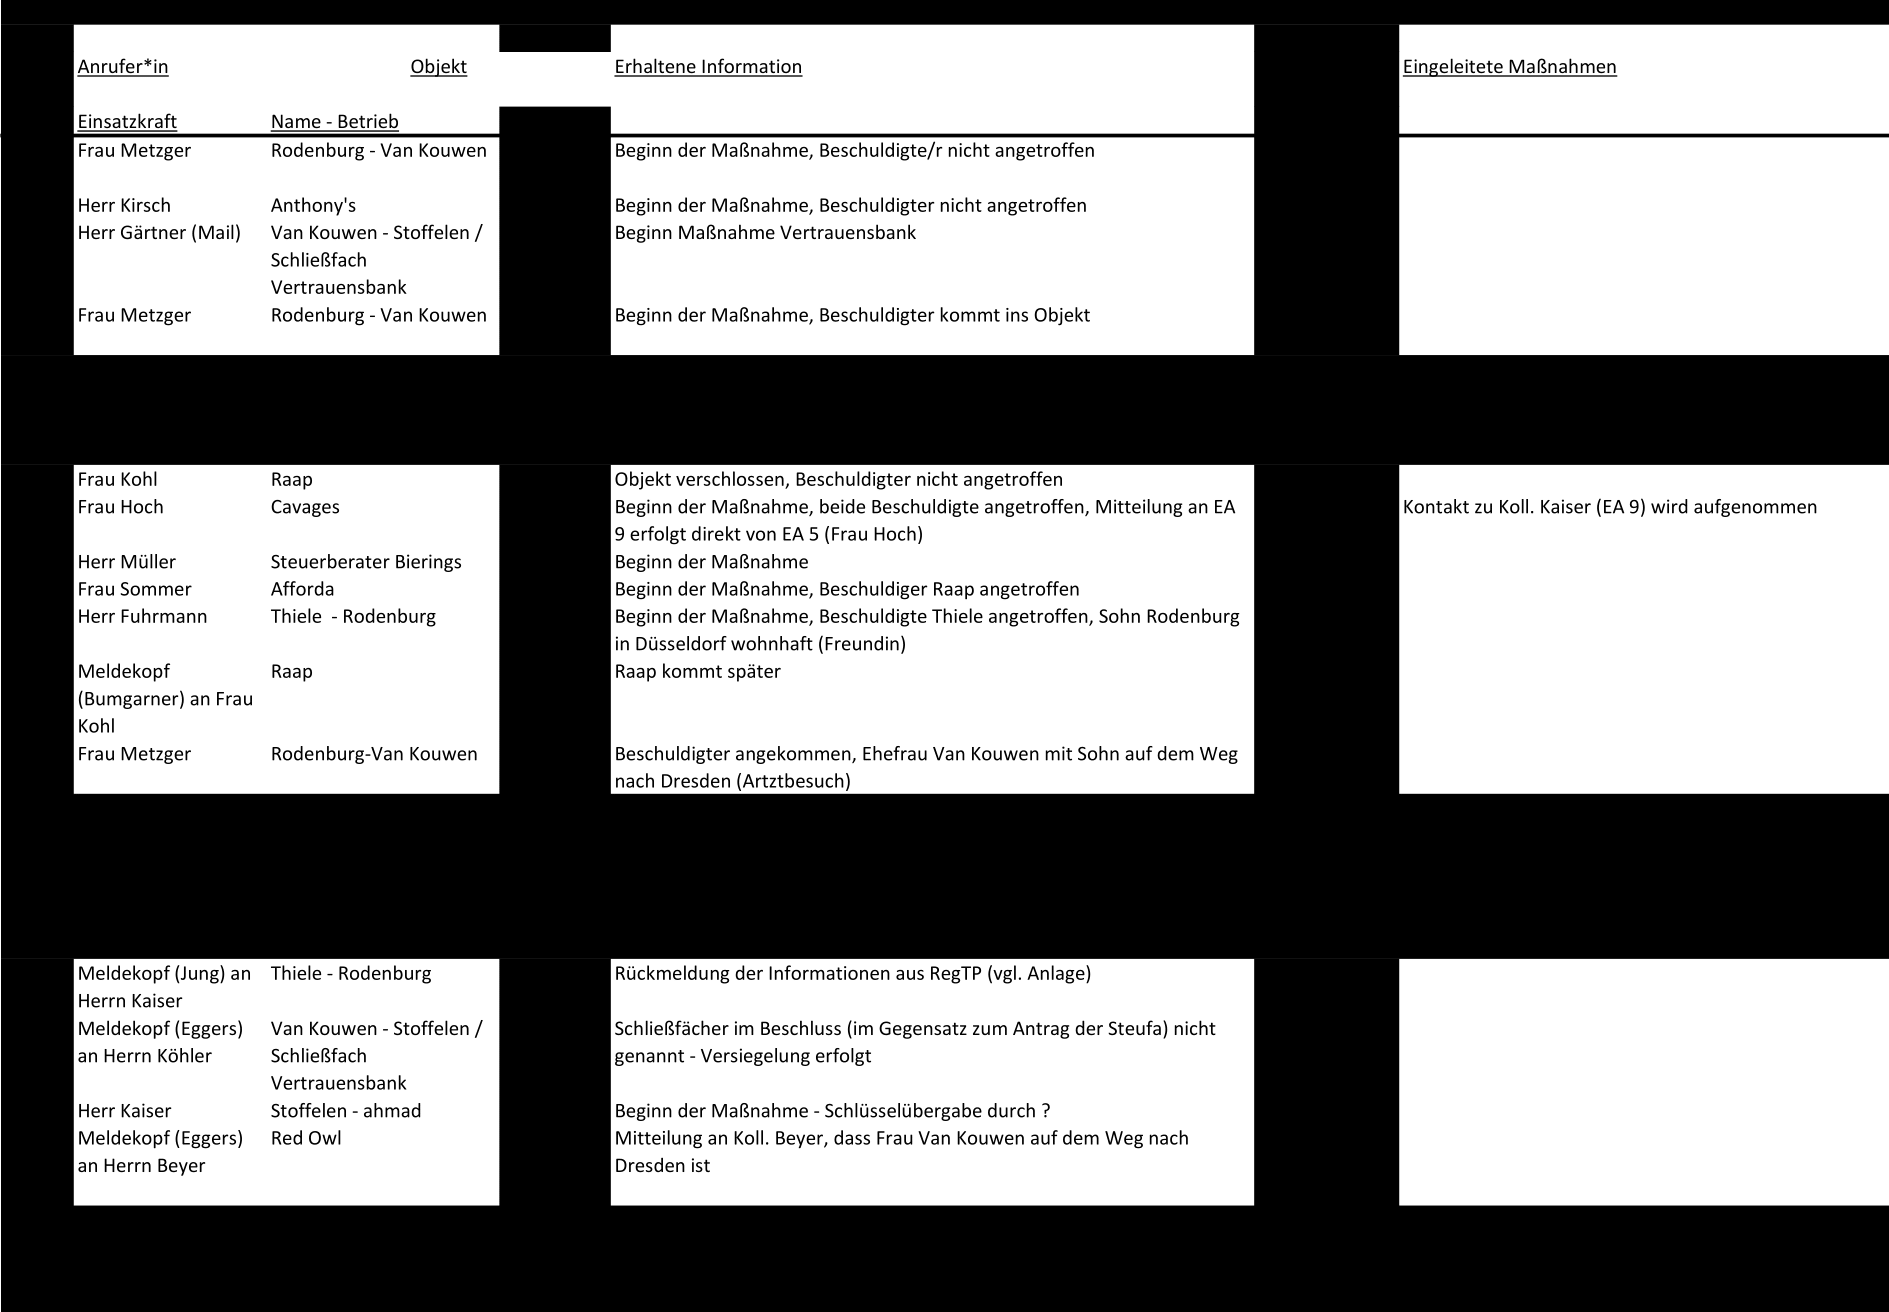
\includegraphics[width=.75\textwidth]{images/0-Artefaktmodell/Chronologie_Meldekopf-1.png}
    \caption{Artefaktmodell Meldekopf (1)}
    \label{fig:chrono1}
\end{figure}

Aus diesem lässt sich erkennen, welche Informationen über Beschuldigte und Objekte im Laufe der Durchsuchung benötigt werden.
Dadurch kann sichergestellt werden, dass das resultierende Produkt nur über die nötigen Funktionen verfügt und keine unhilfreichen Informationen direkt anzeigt.

\begin{figure}[htp]
    \centering
    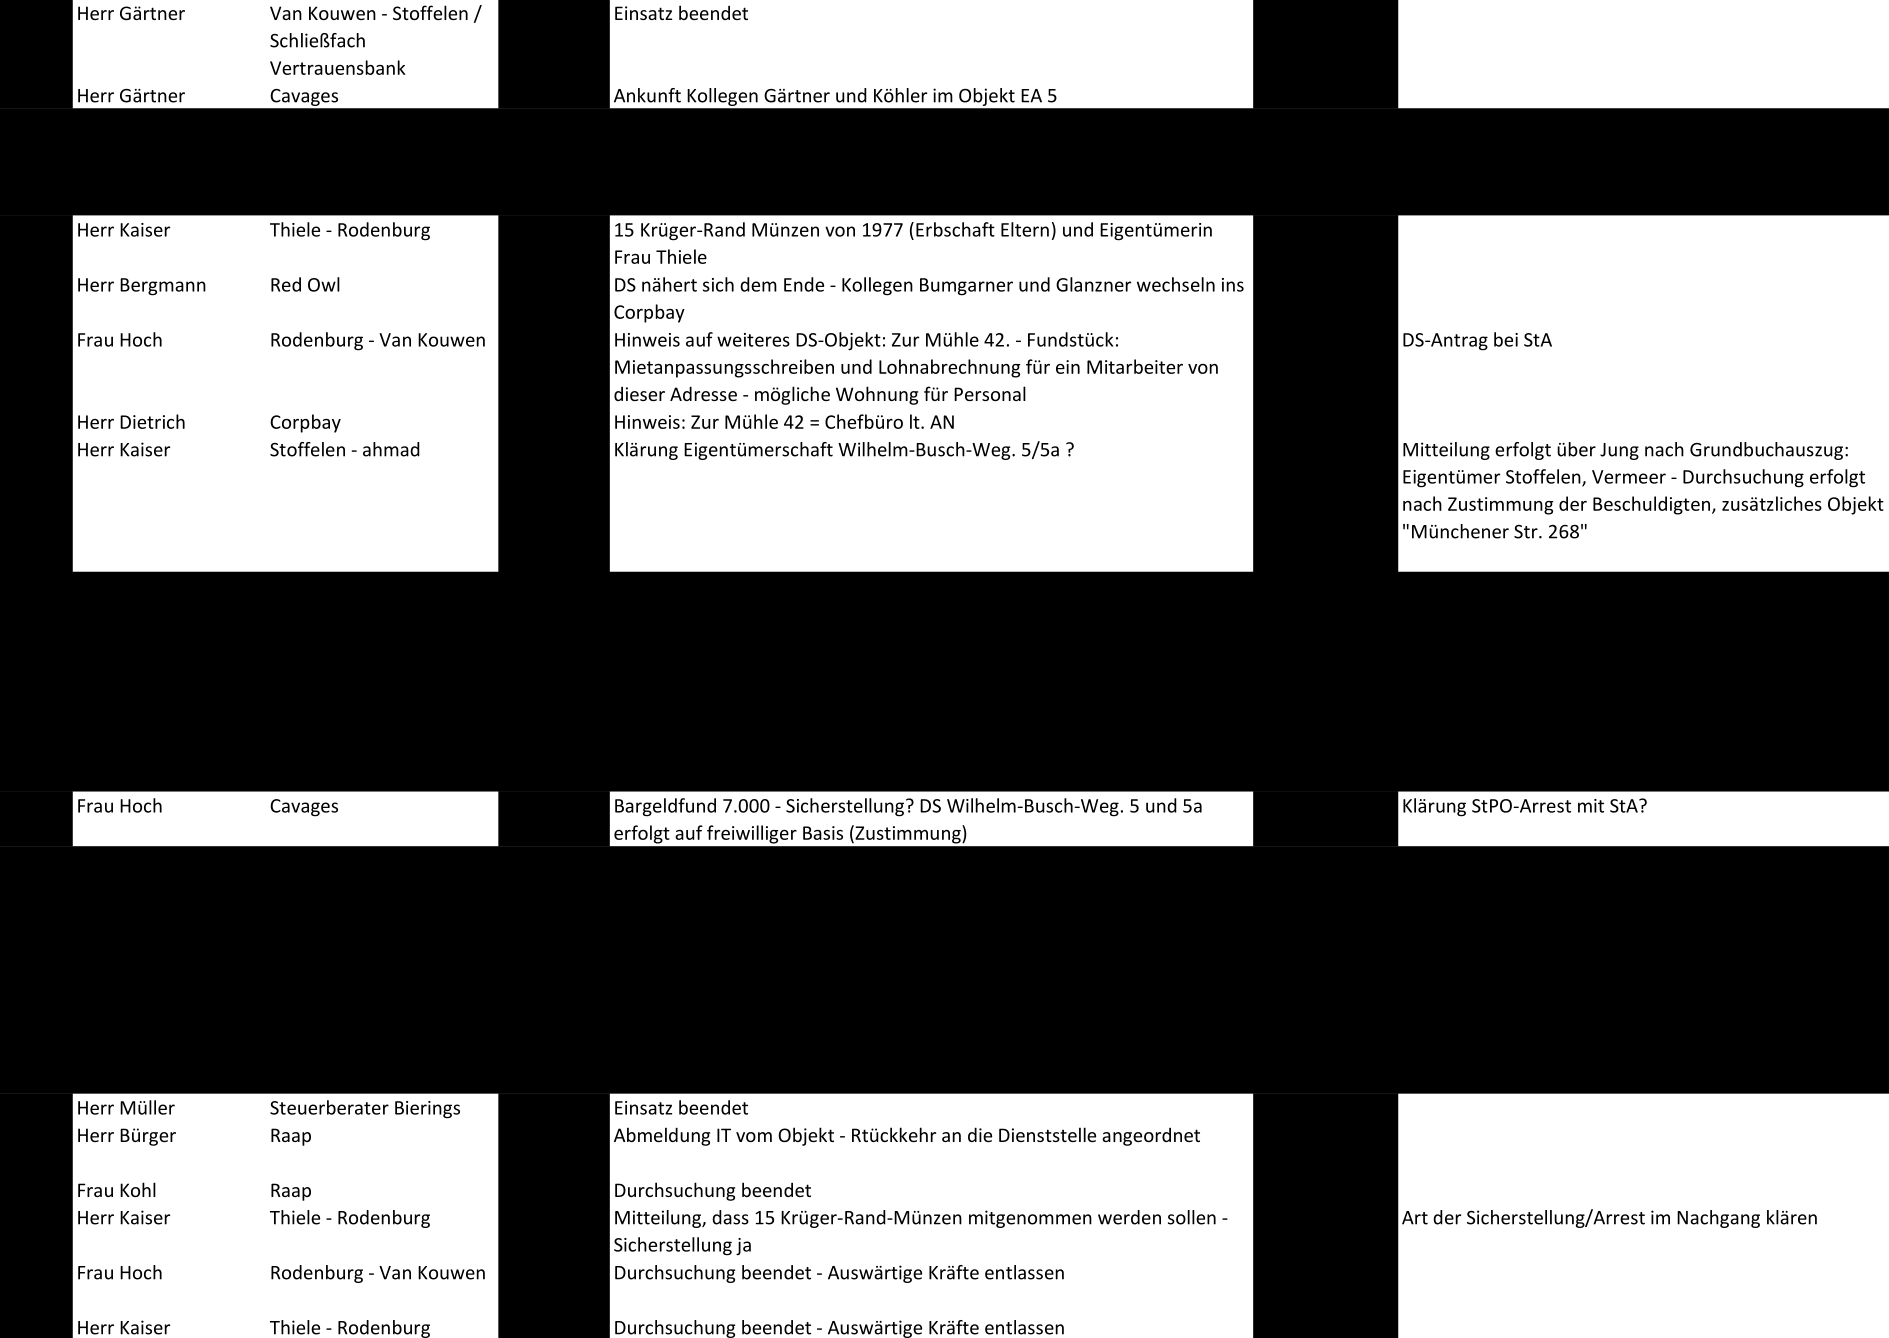
\includegraphics[width=.75\textwidth]{images/0-Artefaktmodell/Chronologie_Meldekopf-2.png}
    \caption{Artefaktmodell Meldekopf (2)}
    \label{fig:chrono2}
\end{figure}

Genauer beschrieben liegt bei dem Modell eine tabellarische Auflistung von Ereignissen der Durchsuchung vor.
Dabei verfügt die Tabelle über die Spalten "AnruferIn", "Objekt", "Erhaltene Informationen" und die optionale Spalte "Eingeleitete Maßnahmen".

Ein zentrale Funktion welche nach der Sichtung des Modells als nötig befunden wurde, im Interview im Kontext jedoch nicht zur Sprache kam ist das spontane Hinzufügen eines neuen Objekts während einer laufenden Durchsuchung.
Enthielte das Produkt diese Funktion nicht, so wäre es im Falle des Auftretens eines neuen Objekts nötig, dieses über die alte, papiergebunde Vorgehensweise zu koordinieren.
Ebenso kann festgestellt werden, dass das Modell nicht über konsistente Syntax innerhalb der Spalten verfügt. 
Am Anfang der zweiten Spalte ist die Überschrift "Name - Betrieb" zu lesen.
Diese Syntax wird zunächst eingehalten, später jedoch verworfen.
Erfahrungsberichte aus dem Interview im Kontext lassen darauf hindeuten, dass dies aus Zeitgründen geschah.

\begin{figure}[htp]
    \centering
    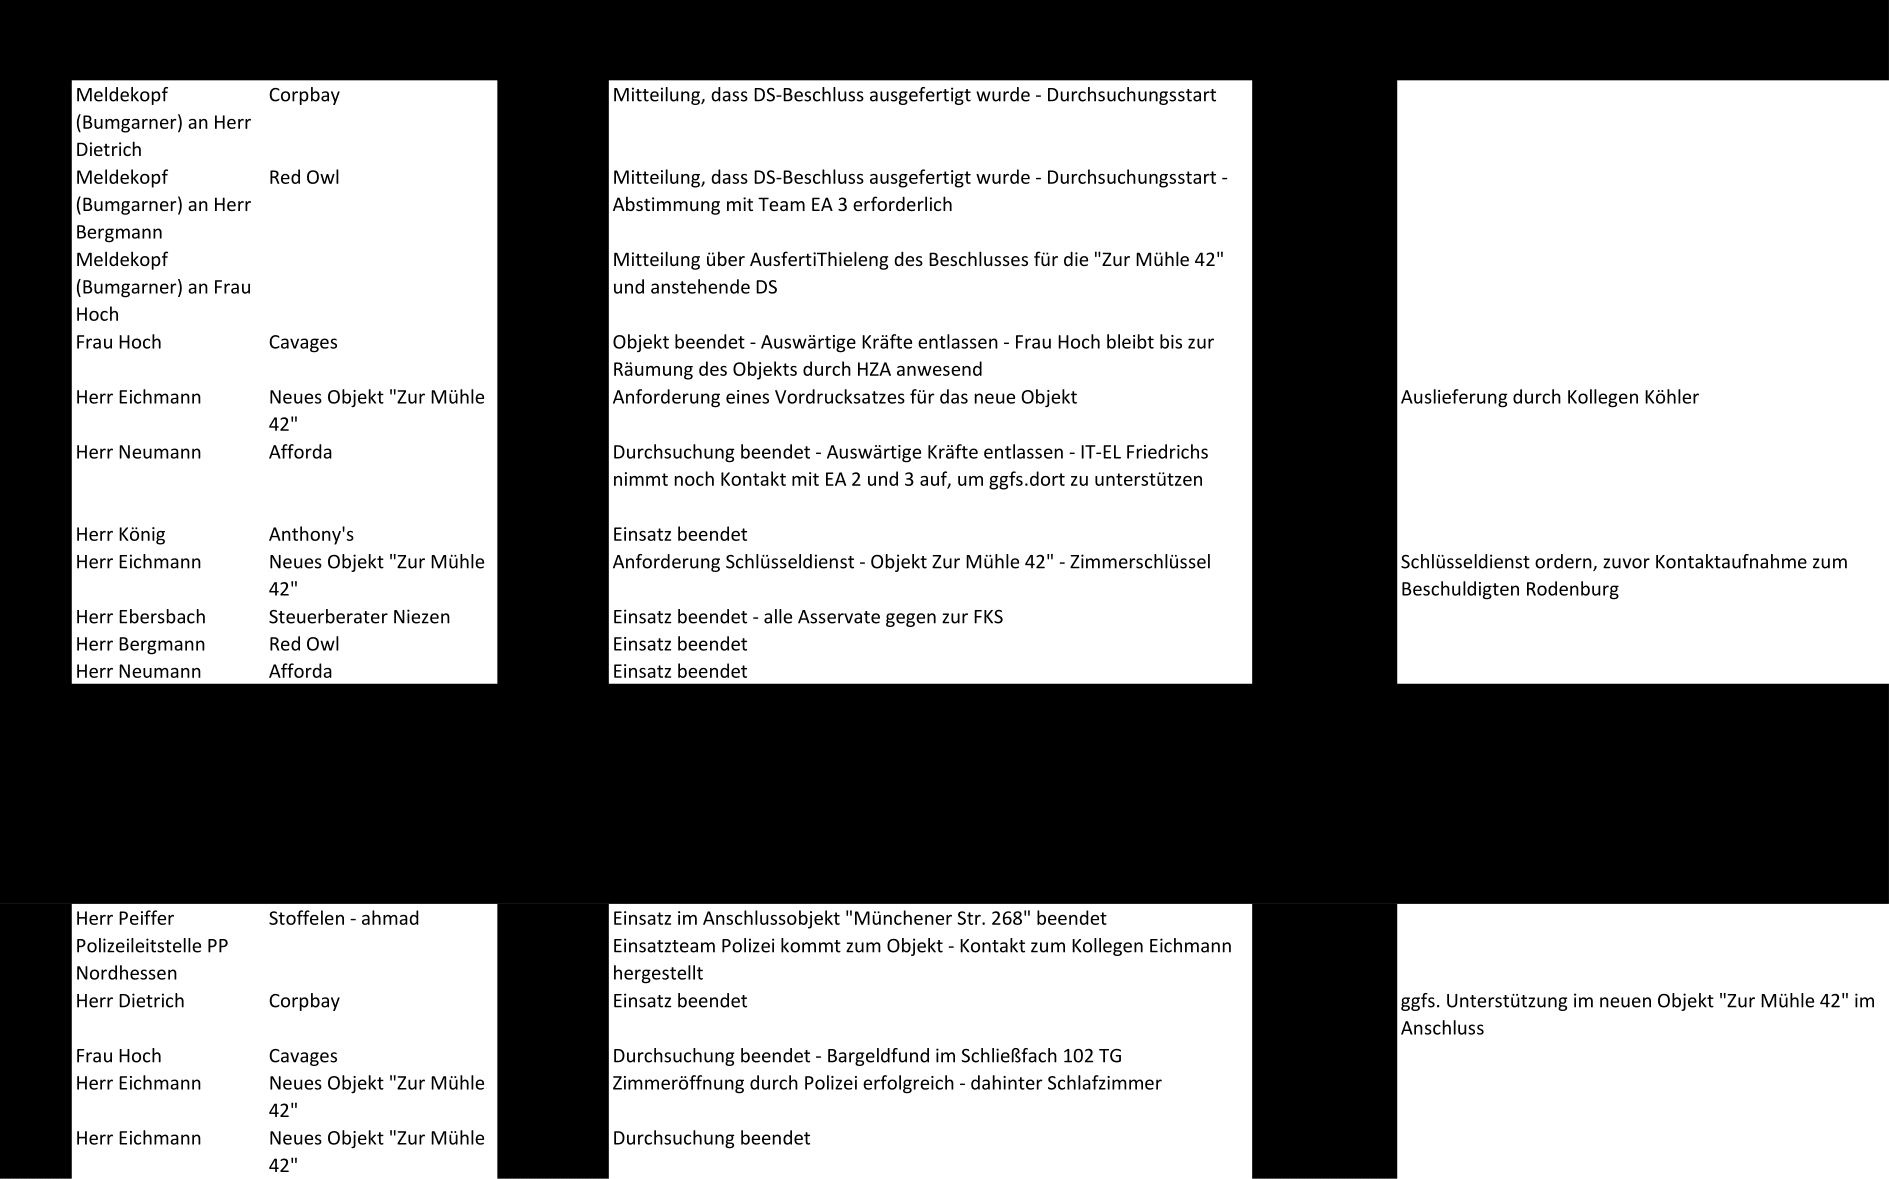
\includegraphics[width=.75\textwidth]{images/0-Artefaktmodell/Chronologie_Meldekopf-3.png}
    \caption{Artefaktmodell Meldekopf (3)}
    \label{fig:chrono3}
\end{figure}

Aus Gründen der Diskretion ist das Artefaktmodell in dieser Abgabe des Dokuments geschwärzt.
Des Weiteren wurden sämtliche Namen geändert und das Dokument gekürzt.
Dies bezieht sich sowohl auf Personen, Betriebe, als auch Straßennamen.
Im Zuge des nutzungsorientieren Prozesses lagen dem Autor jedoch Originaldokumente vor.
